\documentclass[a4paper]{article}

\usepackage[a4paper,width=150mm,top=25mm,bottom=25mm]{geometry}
\usepackage[utf8x]{inputenc}
\usepackage{amsmath}
\usepackage{graphicx}
\usepackage[table]{xcolor}

\title{INTL 450: Advanced Data Analysis in Python}
\author{Alper Yıldırım}

\begin{document}
\maketitle

\section*{Homework 4: Report}

	In this homework assignment, I applied three different machine learning models using two different feature extraction tools to an open-ended survey responses on immigration. The machine learning models were applied to the data set are Support Vector Regression, Random Forest Regression, and Gaussian Process Regression, respectively. Target variable is scaled through \verb|StandardScaler| for the improvement of model performance. The distribution of sentiments is demonstrated in the Figure 1 below.
	
\begin{figure}[htp]
    \centering
    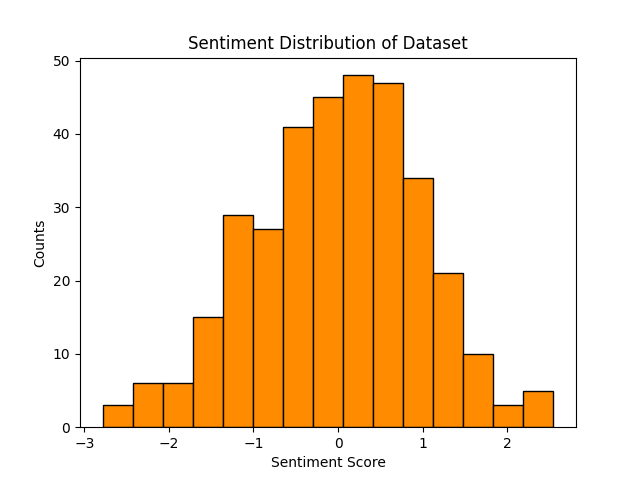
\includegraphics[width=12cm]{sentiment_distribution.png}
    \caption{Sentiment Distribution}
\end{figure}
	
	Except the case of Gaussian Process Regression with \verb|CountVectorizer| using both uni- and bi-grams, all models performed better using uni- and bi-grams, rather than using only bi-grams. Therefore, I fairly conclude that including only bi-grams reduces model performance in this data set. \\

	Moreover, Term Frequency-Inverse Document Frequency (TF-IDF) method performed weaker than \verb|CountVectorizer| in general. Support Vector Regression is the most negatively influenced model with the use of Tf-Idf Vectorizer. On the other hand, Gaussian Process Regression is the only model that performed better with the Tf-Idf Vectorizer with a slight increase in correlation coefficient. In the case of only bi-grams, there is an inverse relationship in correlation coefficients for each model. For instance, while Support Vector Regression has the best performance with 
    \verb|CountVectoizer|, that model performed worst with Tf-Idf Vectorizer. The opposite is correct for the Gaussian Process Regression. \\
	
\begin{table}[htbp!]
\begin{tabular}{ |c|c|c|c| } 
 \hline
 Model & Feature Extraction & Corr. (bigram) & Corr. (uni- \& bigram) \\
 \hline
 Support Vector Regressor & CountVectorizer & 0.510 & 0.684 \\ 
 \hline
 Random Forest Regressor & CountVectorizer & 0.420 & 0.693 \\ 
  \hline
 Gaussian Process Regressor & CountVectorizer & 0.370 & 0.317 \\
 \hline
 Support Vector Regressor & Tf-Idf Vectorizer & 0.300 & 0.503 \\ 
 \hline
 Random Forest Regressor & Tf-Idf Vectorizer & 0.343 & \cellcolor[HTML]{EEAB54}0.706 \\ 
  \hline
 Gaussian Process Regressor & Tf-Idf Vectorizer & 0.395 & 0.571 \\
 \hline
\end{tabular}
\caption{Correlation coefficient for the models}
\end{table} 

    Lastly, the best model performance was achieved through Random Forest Regression including uni- and bi-grams with Tf-Idf Vectorizer. The correlation coefficient, as it is observed in Table 1 above, is equal to 0.706 for that model.

\end{document}